\PassOptionsToPackage{unicode=true}{hyperref} % options for packages loaded elsewhere
\PassOptionsToPackage{hyphens}{url}
%
\documentclass[]{article}
\usepackage{lmodern}
\usepackage{amssymb,amsmath}
\usepackage{ifxetex,ifluatex}
\usepackage{fixltx2e} % provides \textsubscript
\ifnum 0\ifxetex 1\fi\ifluatex 1\fi=0 % if pdftex
  \usepackage[T1]{fontenc}
  \usepackage[utf8]{inputenc}
  \usepackage{textcomp} % provides euro and other symbols
\else % if luatex or xelatex
  \usepackage{unicode-math}
  \defaultfontfeatures{Ligatures=TeX,Scale=MatchLowercase}
\fi
% use upquote if available, for straight quotes in verbatim environments
\IfFileExists{upquote.sty}{\usepackage{upquote}}{}
% use microtype if available
\IfFileExists{microtype.sty}{%
\usepackage[]{microtype}
\UseMicrotypeSet[protrusion]{basicmath} % disable protrusion for tt fonts
}{}
\IfFileExists{parskip.sty}{%
\usepackage{parskip}
}{% else
\setlength{\parindent}{0pt}
\setlength{\parskip}{6pt plus 2pt minus 1pt}
}
\usepackage{hyperref}
\hypersetup{
            pdftitle={Multiple Logistic Regression},
            pdfauthor={SDS 291},
            pdfborder={0 0 0},
            breaklinks=true}
\urlstyle{same}  % don't use monospace font for urls
\usepackage[margin=1in]{geometry}
\usepackage{color}
\usepackage{fancyvrb}
\newcommand{\VerbBar}{|}
\newcommand{\VERB}{\Verb[commandchars=\\\{\}]}
\DefineVerbatimEnvironment{Highlighting}{Verbatim}{commandchars=\\\{\}}
% Add ',fontsize=\small' for more characters per line
\usepackage{framed}
\definecolor{shadecolor}{RGB}{248,248,248}
\newenvironment{Shaded}{\begin{snugshade}}{\end{snugshade}}
\newcommand{\AlertTok}[1]{\textcolor[rgb]{0.94,0.16,0.16}{#1}}
\newcommand{\AnnotationTok}[1]{\textcolor[rgb]{0.56,0.35,0.01}{\textbf{\textit{#1}}}}
\newcommand{\AttributeTok}[1]{\textcolor[rgb]{0.77,0.63,0.00}{#1}}
\newcommand{\BaseNTok}[1]{\textcolor[rgb]{0.00,0.00,0.81}{#1}}
\newcommand{\BuiltInTok}[1]{#1}
\newcommand{\CharTok}[1]{\textcolor[rgb]{0.31,0.60,0.02}{#1}}
\newcommand{\CommentTok}[1]{\textcolor[rgb]{0.56,0.35,0.01}{\textit{#1}}}
\newcommand{\CommentVarTok}[1]{\textcolor[rgb]{0.56,0.35,0.01}{\textbf{\textit{#1}}}}
\newcommand{\ConstantTok}[1]{\textcolor[rgb]{0.00,0.00,0.00}{#1}}
\newcommand{\ControlFlowTok}[1]{\textcolor[rgb]{0.13,0.29,0.53}{\textbf{#1}}}
\newcommand{\DataTypeTok}[1]{\textcolor[rgb]{0.13,0.29,0.53}{#1}}
\newcommand{\DecValTok}[1]{\textcolor[rgb]{0.00,0.00,0.81}{#1}}
\newcommand{\DocumentationTok}[1]{\textcolor[rgb]{0.56,0.35,0.01}{\textbf{\textit{#1}}}}
\newcommand{\ErrorTok}[1]{\textcolor[rgb]{0.64,0.00,0.00}{\textbf{#1}}}
\newcommand{\ExtensionTok}[1]{#1}
\newcommand{\FloatTok}[1]{\textcolor[rgb]{0.00,0.00,0.81}{#1}}
\newcommand{\FunctionTok}[1]{\textcolor[rgb]{0.00,0.00,0.00}{#1}}
\newcommand{\ImportTok}[1]{#1}
\newcommand{\InformationTok}[1]{\textcolor[rgb]{0.56,0.35,0.01}{\textbf{\textit{#1}}}}
\newcommand{\KeywordTok}[1]{\textcolor[rgb]{0.13,0.29,0.53}{\textbf{#1}}}
\newcommand{\NormalTok}[1]{#1}
\newcommand{\OperatorTok}[1]{\textcolor[rgb]{0.81,0.36,0.00}{\textbf{#1}}}
\newcommand{\OtherTok}[1]{\textcolor[rgb]{0.56,0.35,0.01}{#1}}
\newcommand{\PreprocessorTok}[1]{\textcolor[rgb]{0.56,0.35,0.01}{\textit{#1}}}
\newcommand{\RegionMarkerTok}[1]{#1}
\newcommand{\SpecialCharTok}[1]{\textcolor[rgb]{0.00,0.00,0.00}{#1}}
\newcommand{\SpecialStringTok}[1]{\textcolor[rgb]{0.31,0.60,0.02}{#1}}
\newcommand{\StringTok}[1]{\textcolor[rgb]{0.31,0.60,0.02}{#1}}
\newcommand{\VariableTok}[1]{\textcolor[rgb]{0.00,0.00,0.00}{#1}}
\newcommand{\VerbatimStringTok}[1]{\textcolor[rgb]{0.31,0.60,0.02}{#1}}
\newcommand{\WarningTok}[1]{\textcolor[rgb]{0.56,0.35,0.01}{\textbf{\textit{#1}}}}
\usepackage{graphicx,grffile}
\makeatletter
\def\maxwidth{\ifdim\Gin@nat@width>\linewidth\linewidth\else\Gin@nat@width\fi}
\def\maxheight{\ifdim\Gin@nat@height>\textheight\textheight\else\Gin@nat@height\fi}
\makeatother
% Scale images if necessary, so that they will not overflow the page
% margins by default, and it is still possible to overwrite the defaults
% using explicit options in \includegraphics[width, height, ...]{}
\setkeys{Gin}{width=\maxwidth,height=\maxheight,keepaspectratio}
\setlength{\emergencystretch}{3em}  % prevent overfull lines
\providecommand{\tightlist}{%
  \setlength{\itemsep}{0pt}\setlength{\parskip}{0pt}}
\setcounter{secnumdepth}{0}
% Redefines (sub)paragraphs to behave more like sections
\ifx\paragraph\undefined\else
\let\oldparagraph\paragraph
\renewcommand{\paragraph}[1]{\oldparagraph{#1}\mbox{}}
\fi
\ifx\subparagraph\undefined\else
\let\oldsubparagraph\subparagraph
\renewcommand{\subparagraph}[1]{\oldsubparagraph{#1}\mbox{}}
\fi

% set default figure placement to htbp
\makeatletter
\def\fps@figure{htbp}
\makeatother


\title{Multiple Logistic Regression}
\author{SDS 291}
\date{April 15, 2020}

\begin{document}
\maketitle

We're going to work with the \texttt{Whickham} data contains
observations about women, and whether they were alive 20 years after
their initial observation (\texttt{outcome} is a 2 level factor variable
- Alive/Dead). You can learn more about these data from the
\texttt{mosaicData} help feature if you'd like.

Specifically, we're interested in: the association of age, smoking
status (smoker), and 20-year survival (outcome: alive (success), dead
(reference / failure)). Bring in the relevant packages and the data
(below, from the mosaic package).

\begin{Shaded}
\begin{Highlighting}[]
\KeywordTok{library}\NormalTok{(mosaic)}
\KeywordTok{library}\NormalTok{(tidyverse)}
\KeywordTok{data}\NormalTok{(}\StringTok{"Whickham"}\NormalTok{)}
\NormalTok{Whickham}\OperatorTok{$}\NormalTok{outcome<-}\KeywordTok{relevel}\NormalTok{(Whickham}\OperatorTok{$}\NormalTok{outcome, }\DataTypeTok{ref=}\StringTok{"Dead"}\NormalTok{)}
\end{Highlighting}
\end{Shaded}

\newpage

\hypertarget{age-and-outcome}{%
\section{Age and Outcome}\label{age-and-outcome}}

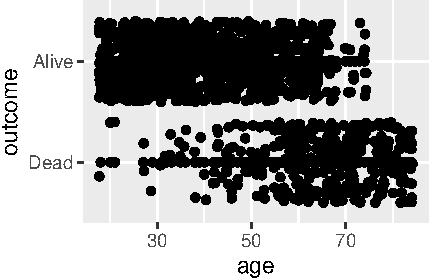
\includegraphics{20-inclasslab_files/figure-latex/unnamed-chunk-3-1.pdf}
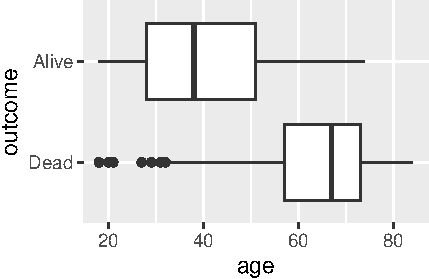
\includegraphics{20-inclasslab_files/figure-latex/unnamed-chunk-3-2.pdf}

\begin{Shaded}
\begin{Highlighting}[]
\NormalTok{m0<-}\KeywordTok{glm}\NormalTok{(outcome}\OperatorTok{~}\NormalTok{age, }\DataTypeTok{data=}\NormalTok{Whickham, }\DataTypeTok{family=}\NormalTok{binomial)}
\KeywordTok{summary}\NormalTok{(m0)}
\end{Highlighting}
\end{Shaded}

\begin{verbatim}
## 
## Call:
## glm(formula = outcome ~ age, family = binomial, data = Whickham)
## 
## Deviance Residuals: 
##     Min       1Q   Median       3Q      Max  
## -3.2296  -0.4277   0.2293   0.5538   1.8953  
## 
## Coefficients:
##              Estimate Std. Error z value Pr(>|z|)    
## (Intercept)  7.403126   0.403522   18.35   <2e-16 ***
## age         -0.121861   0.006941  -17.56   <2e-16 ***
## ---
## Signif. codes:  0 '***' 0.001 '**' 0.01 '*' 0.05 '.' 0.1 ' ' 1
## 
## (Dispersion parameter for binomial family taken to be 1)
## 
##     Null deviance: 1560.32  on 1313  degrees of freedom
## Residual deviance:  946.51  on 1312  degrees of freedom
## AIC: 950.51
## 
## Number of Fisher Scoring iterations: 6
\end{verbatim}

\begin{enumerate}
\def\labelenumi{\arabic{enumi}.}
\tightlist
\item
  Write the fitted equation and interpret the results (in these units)
  in light of the question. Be sure to comment on the magnitude and
  direction of the association.
\end{enumerate}

\vspace{1in}

\begin{enumerate}
\def\labelenumi{\arabic{enumi}.}
\setcounter{enumi}{1}
\tightlist
\item
  Based on this model, what is the probability that a 60 year old was
  alive 20 years after the initial survey?
\end{enumerate}

\vspace{2in}

\newpage

\hypertarget{smoking-status-and-outcome-alive}{%
\section{Smoking Status and Outcome
(Alive)}\label{smoking-status-and-outcome-alive}}

\begin{Shaded}
\begin{Highlighting}[]
\NormalTok{Whickham}\OperatorTok{$}\NormalTok{smoker<-}\KeywordTok{factor}\NormalTok{(Whickham}\OperatorTok{$}\NormalTok{smoker, }\DataTypeTok{levels=}\KeywordTok{c}\NormalTok{(}\StringTok{"Yes"}\NormalTok{, }\StringTok{"No"}\NormalTok{))}
\NormalTok{Whickham}\OperatorTok{$}\NormalTok{outcome<-}\KeywordTok{factor}\NormalTok{(Whickham}\OperatorTok{$}\NormalTok{outcome, }\DataTypeTok{levels=}\KeywordTok{c}\NormalTok{(}\StringTok{"Alive"}\NormalTok{, }\StringTok{"Dead"}\NormalTok{))}
\KeywordTok{tally}\NormalTok{(}\OperatorTok{~}\StringTok{ }\NormalTok{smoker }\OperatorTok{+}\StringTok{ }\NormalTok{outcome, }\DataTypeTok{margins=}\OtherTok{FALSE}\NormalTok{, }\DataTypeTok{data=}\NormalTok{Whickham)}
\end{Highlighting}
\end{Shaded}

\begin{verbatim}
##       outcome
## smoker Alive Dead
##    Yes   443  139
##    No    502  230
\end{verbatim}

\begin{enumerate}
\def\labelenumi{\arabic{enumi}.}
\setcounter{enumi}{2}
\tightlist
\item
  Calculate the Odds Ratio of non-smokers being alive in 20 years
  compared to smokers from the table above. \vspace{3in}
\end{enumerate}

\begin{Shaded}
\begin{Highlighting}[]
\NormalTok{Whickham}\OperatorTok{$}\NormalTok{smoker<-}\KeywordTok{relevel}\NormalTok{(Whickham}\OperatorTok{$}\NormalTok{smoker, }\DataTypeTok{ref=} \StringTok{"No"}\NormalTok{)}
\NormalTok{Whickham}\OperatorTok{$}\NormalTok{outcome<-}\KeywordTok{relevel}\NormalTok{(Whickham}\OperatorTok{$}\NormalTok{outcome, }\DataTypeTok{ref=} \StringTok{"Dead"}\NormalTok{)}
\NormalTok{m1<-}\KeywordTok{glm}\NormalTok{(outcome}\OperatorTok{~}\NormalTok{smoker, }\DataTypeTok{data=}\NormalTok{Whickham, }\DataTypeTok{family=}\NormalTok{binomial)}
\KeywordTok{summary}\NormalTok{(m1)}
\end{Highlighting}
\end{Shaded}

\begin{verbatim}
## 
## Call:
## glm(formula = outcome ~ smoker, family = binomial, data = Whickham)
## 
## Deviance Residuals: 
##     Min       1Q   Median       3Q      Max  
## -1.6923  -1.5216   0.7388   0.8685   0.8685  
## 
## Coefficients:
##             Estimate Std. Error z value Pr(>|z|)    
## (Intercept)  0.78052    0.07962   9.803  < 2e-16 ***
## smokerYes    0.37858    0.12566   3.013  0.00259 ** 
## ---
## Signif. codes:  0 '***' 0.001 '**' 0.01 '*' 0.05 '.' 0.1 ' ' 1
## 
## (Dispersion parameter for binomial family taken to be 1)
## 
##     Null deviance: 1560.3  on 1313  degrees of freedom
## Residual deviance: 1551.1  on 1312  degrees of freedom
## AIC: 1555.1
## 
## Number of Fisher Scoring iterations: 4
\end{verbatim}

\begin{enumerate}
\def\labelenumi{\arabic{enumi}.}
\setcounter{enumi}{3}
\tightlist
\item
  Show that you can calculate the coefficient for smoking status from
  your regression model as you did in \#3.
\end{enumerate}

\vspace{3in}

\begin{enumerate}
\def\labelenumi{\arabic{enumi}.}
\setcounter{enumi}{4}
\tightlist
\item
  Based on your model, what's the probability that a smoker was alive 20
  years later?
\end{enumerate}

\vspace{3in}

\begin{enumerate}
\def\labelenumi{\arabic{enumi}.}
\setcounter{enumi}{5}
\tightlist
\item
  Based on what you know about the risk of death for age and smoking
  status, do these results make sense? Explain your answer.
\end{enumerate}

\newpage

\hypertarget{multiple-logistic-regression}{%
\subsection{Multiple Logistic
Regression}\label{multiple-logistic-regression}}

\begin{Shaded}
\begin{Highlighting}[]
\NormalTok{m2<-}\KeywordTok{glm}\NormalTok{(outcome}\OperatorTok{~}\NormalTok{age}\OperatorTok{+}\NormalTok{smoker, }\DataTypeTok{data=}\NormalTok{Whickham, }\DataTypeTok{family=}\NormalTok{binomial)}
\KeywordTok{summary}\NormalTok{(m2)}
\end{Highlighting}
\end{Shaded}

\begin{verbatim}
## 
## Call:
## glm(formula = outcome ~ age + smoker, family = binomial, data = Whickham)
## 
## Deviance Residuals: 
##     Min       1Q   Median       3Q      Max  
## -3.2795  -0.4381   0.2228   0.5458   1.9581  
## 
## Coefficients:
##              Estimate Std. Error z value Pr(>|z|)    
## (Intercept)  7.599221   0.441231  17.223   <2e-16 ***
## age         -0.123683   0.007177 -17.233   <2e-16 ***
## smokerYes   -0.204699   0.168422  -1.215    0.224    
## ---
## Signif. codes:  0 '***' 0.001 '**' 0.01 '*' 0.05 '.' 0.1 ' ' 1
## 
## (Dispersion parameter for binomial family taken to be 1)
## 
##     Null deviance: 1560.32  on 1313  degrees of freedom
## Residual deviance:  945.02  on 1311  degrees of freedom
## AIC: 951.02
## 
## Number of Fisher Scoring iterations: 6
\end{verbatim}

\begin{enumerate}
\def\labelenumi{\arabic{enumi}.}
\setcounter{enumi}{6}
\tightlist
\item
  What is the odds ratio for smokers compared to non-smokers in this
  model? Interpret in a sentence in the context of this real-world
  problem.
\end{enumerate}

\vspace{3in}

\begin{enumerate}
\def\labelenumi{\arabic{enumi}.}
\setcounter{enumi}{7}
\tightlist
\item
  What is the probability of a 60 year old non-smoker being alive 20
  years later?
\end{enumerate}

\vspace{3in}

\begin{enumerate}
\def\labelenumi{\arabic{enumi}.}
\setcounter{enumi}{8}
\tightlist
\item
  What is the probability of a 40 year old smoker being alive 20 years
  later?
\end{enumerate}

\vspace{3in}

\begin{enumerate}
\def\labelenumi{\arabic{enumi}.}
\setcounter{enumi}{9}
\tightlist
\item
  What does this model help us to understand about our simple logistic
  regression estimates above?
\end{enumerate}

\vspace{3in}

\hypertarget{optional---interaction-term}{%
\subsubsection{\texorpdfstring{\emph{Optional} - Interaction
Term}{Optional - Interaction Term}}\label{optional---interaction-term}}

\begin{enumerate}
\def\labelenumi{\arabic{enumi}.}
\setcounter{enumi}{10}
\tightlist
\item
  What would an interaction term between age and smoking status do in
  this model? How would an interaction term affect the OR for age?
\end{enumerate}

\vspace{3in}

\begin{enumerate}
\def\labelenumi{\arabic{enumi}.}
\setcounter{enumi}{11}
\tightlist
\item
  How do the coefficients in the interaction model relate to the
  separate models for Age for smokers and non-smokers (below)?
\end{enumerate}

\vspace{0.5in}

\hypertarget{interaction}{%
\paragraph{Interaction}\label{interaction}}

\begin{Shaded}
\begin{Highlighting}[]
\NormalTok{m3<-}\KeywordTok{glm}\NormalTok{(outcome}\OperatorTok{~}\NormalTok{age}\OperatorTok{+}\NormalTok{smoker}\OperatorTok{+}\NormalTok{age}\OperatorTok{*}\NormalTok{smoker, }\DataTypeTok{data=}\NormalTok{Whickham, }\DataTypeTok{family=}\NormalTok{binomial)}
\KeywordTok{summary}\NormalTok{(m3)}
\end{Highlighting}
\end{Shaded}

\begin{verbatim}
## 
## Call:
## glm(formula = outcome ~ age + smoker + age * smoker, family = binomial, 
##     data = Whickham)
## 
## Deviance Residuals: 
##     Min       1Q   Median       3Q      Max  
## -3.3983  -0.4256   0.2163   0.5598   1.9283  
## 
## Coefficients:
##                Estimate Std. Error z value Pr(>|z|)    
## (Intercept)    8.169231   0.606600  13.467   <2e-16 ***
## age           -0.133231   0.009953 -13.386   <2e-16 ***
## smokerYes     -1.457843   0.837232  -1.741   0.0816 .  
## age:smokerYes  0.022235   0.014495   1.534   0.1250    
## ---
## Signif. codes:  0 '***' 0.001 '**' 0.01 '*' 0.05 '.' 0.1 ' ' 1
## 
## (Dispersion parameter for binomial family taken to be 1)
## 
##     Null deviance: 1560.32  on 1313  degrees of freedom
## Residual deviance:  942.68  on 1310  degrees of freedom
## AIC: 950.68
## 
## Number of Fisher Scoring iterations: 6
\end{verbatim}

\hypertarget{smokers}{%
\paragraph{Smokers}\label{smokers}}

\begin{Shaded}
\begin{Highlighting}[]
\NormalTok{Whickham_smoker<-}\StringTok{ }\NormalTok{Whickham }\OperatorTok\StringTok{ }\KeywordTok{filter}\NormalTok{(smoker}\OperatorTok{==}\StringTok{"Yes"}\NormalTok{)}
\NormalTok{m3_smoker<-}\KeywordTok{glm}\NormalTok{(outcome}\OperatorTok{~}\NormalTok{age, }\DataTypeTok{data=}\NormalTok{Whickham_smoker, }\DataTypeTok{family=}\NormalTok{binomial)}
\KeywordTok{summary}\NormalTok{(m3_smoker)}
\end{Highlighting}
\end{Shaded}

\begin{verbatim}
## 
## Call:
## glm(formula = outcome ~ age, family = binomial, data = Whickham_smoker)
## 
## Deviance Residuals: 
##     Min       1Q   Median       3Q      Max  
## -3.0009   0.1337   0.3044   0.6362   1.8457  
## 
## Coefficients:
##             Estimate Std. Error z value Pr(>|z|)    
## (Intercept)  6.71139    0.57702   11.63   <2e-16 ***
## age         -0.11100    0.01054  -10.53   <2e-16 ***
## ---
## Signif. codes:  0 '***' 0.001 '**' 0.01 '*' 0.05 '.' 0.1 ' ' 1
## 
## (Dispersion parameter for binomial family taken to be 1)
## 
##     Null deviance: 639.89  on 581  degrees of freedom
## Residual deviance: 453.72  on 580  degrees of freedom
## AIC: 457.72
## 
## Number of Fisher Scoring iterations: 5
\end{verbatim}

\hypertarget{non-smokers}{%
\paragraph{Non-Smokers}\label{non-smokers}}

\begin{Shaded}
\begin{Highlighting}[]
\NormalTok{Whickham_nonsmoker<-}\StringTok{ }\NormalTok{Whickham }\OperatorTok\StringTok{ }\KeywordTok{filter}\NormalTok{(smoker}\OperatorTok{==}\StringTok{"No"}\NormalTok{)}
\NormalTok{m3_nonsmoker<-}\KeywordTok{glm}\NormalTok{(outcome}\OperatorTok{~}\NormalTok{age, }\DataTypeTok{data=}\NormalTok{Whickham_nonsmoker, }\DataTypeTok{family=}\NormalTok{binomial)}
\KeywordTok{summary}\NormalTok{(m3_nonsmoker)}
\end{Highlighting}
\end{Shaded}

\begin{verbatim}
## 
## Call:
## glm(formula = outcome ~ age, family = binomial, data = Whickham_nonsmoker)
## 
## Deviance Residuals: 
##     Min       1Q   Median       3Q      Max  
## -3.3983  -0.4609   0.1532   0.4357   1.9283  
## 
## Coefficients:
##              Estimate Std. Error z value Pr(>|z|)    
## (Intercept)  8.169231   0.606600   13.47   <2e-16 ***
## age         -0.133231   0.009953  -13.39   <2e-16 ***
## ---
## Signif. codes:  0 '***' 0.001 '**' 0.01 '*' 0.05 '.' 0.1 ' ' 1
## 
## (Dispersion parameter for binomial family taken to be 1)
## 
##     Null deviance: 911.23  on 731  degrees of freedom
## Residual deviance: 488.96  on 730  degrees of freedom
## AIC: 492.96
## 
## Number of Fisher Scoring iterations: 6
\end{verbatim}

\vspace{3in}

\begin{enumerate}
\def\labelenumi{\arabic{enumi}.}
\setcounter{enumi}{12}
\tightlist
\item
  Is this model with the interaction term a better fit than the model
  with Age alone (Model 0 above), or than the model with just Smoking
  alone (Model 1)?
\end{enumerate}

\begin{Shaded}
\begin{Highlighting}[]
\KeywordTok{library}\NormalTok{(lmtest)}
\KeywordTok{lrtest}\NormalTok{(m3,m0)}
\end{Highlighting}
\end{Shaded}

\begin{verbatim}
## Likelihood ratio test
## 
## Model 1: outcome ~ age + smoker + age * smoker
## Model 2: outcome ~ age
##   #Df  LogLik Df  Chisq Pr(>Chisq)
## 1   4 -471.34                     
## 2   2 -473.25 -2 3.8255     0.1477
\end{verbatim}

\begin{Shaded}
\begin{Highlighting}[]
\KeywordTok{lrtest}\NormalTok{(m3,m1)}
\end{Highlighting}
\end{Shaded}

\begin{verbatim}
## Likelihood ratio test
## 
## Model 1: outcome ~ age + smoker + age * smoker
## Model 2: outcome ~ smoker
##   #Df  LogLik Df  Chisq Pr(>Chisq)    
## 1   4 -471.34                         
## 2   2 -775.56 -2 608.44  < 2.2e-16 ***
## ---
## Signif. codes:  0 '***' 0.001 '**' 0.01 '*' 0.05 '.' 0.1 ' ' 1
\end{verbatim}

\begin{enumerate}
\def\labelenumi{\alph{enumi}.}
\item
  What are the null and alternative hypotheses for each of these tests?
  \vspace{2in}
\item
  What is the test statistic and p-value for each and what does that
  mean about the test?
\end{enumerate}

\vspace{2in}

\begin{enumerate}
\def\labelenumi{\alph{enumi}.}
\setcounter{enumi}{2}
\tightlist
\item
  What do these tests tell you about the relationships between age,
  smoking, and survival over 20 years in this cohort of women from
  Whickham? \vspace{2in}
\end{enumerate}

\end{document}
